%!TEX root = ../assignment2.tex

\section{Deployment Plan}

After collecting and analyzing the data from transcripts of interviews, proposing candidate solutions and evaluating them, the deployment plan is ready to be presented, which consists of a goal, issues, solutions and the evaluated solutions in a hierarchical structure with connections linked from the top to the bottom shown in \autoref{img:hier}.

\begin{figure}[ht]
\centering
\caption{Hierarchy of Planning}
\resizebox{\columnwidth}{!}{%
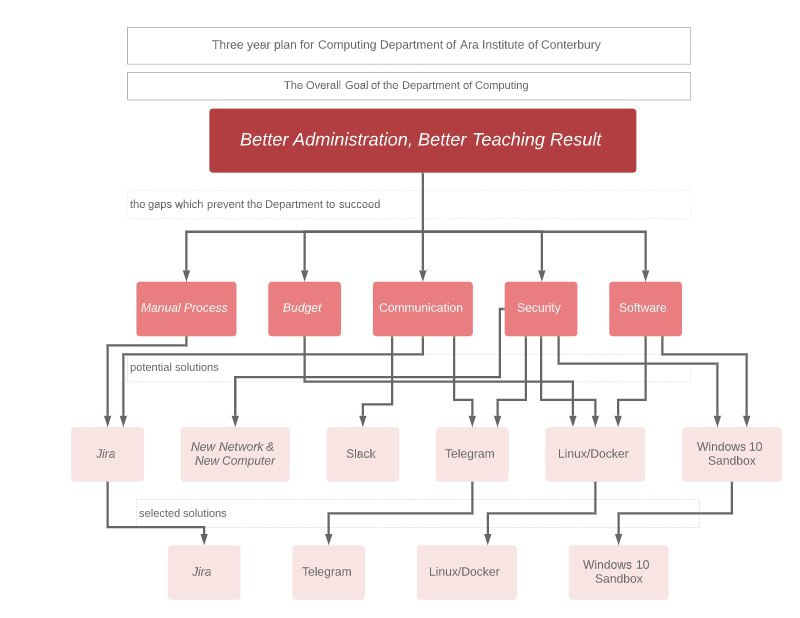
\includegraphics{hierarchy.jpg}
}
\label{img:hier}
\end{figure}
% In this section, we gather the findings of two phases of research and seek to invent a general tool for partitioners to evaluate how possible a IT project is going to succeed.


% \subsection{Summary of Findings}
% There are 21 solutions for control, 11 for people, 7 for process and 5 for structure in both phases. The same primary themes(control, people, process, structure) are used for tagging the gaps and solutions in both phases, which indicates that there is a similarity among the articles. To further investigate the agreement and the difference between the findings, we use mathematical approaches to investigate the agreement of the findings in both phases.

% \subsubsection{Average and Standard Deviation}
% In Phase 1, the average global influence score is 3.6 and the standard deviation is 2.17. In Phase 2, they are 2.66 and 1.37. It suggests the proposals in Phase 1 has a more general influence on how to make IT deployment project successful. However, standard deviation values indicate the influence of power in Phase 1 varies more than that of Phase 2.
% \subsubsection{Pie Chart by Primary Themes}
% To further our analysis on how primary themes(control, process, people and structure) distribute in both Phase 1 and Phase 2, we draw a pie chart to show the proportion.

% \begin{figure}[!ht]
% \centering
% \begin{minipage}{.5\textwidth}
%   \centering
%   %\includegraphics[width=.5\linewidth]{pie_chart_p1.png}
%   \includegraphics[height=10em]{pie_chart_p1.png}
%   \captionof{figure}{Primary Themes in Phase 1}
%   \label{pie:1}
% \end{minipage}%
% \begin{minipage}{.5\textwidth}
%   \centering
%   %\includegraphics[width=.5\linewidth]{pie_chart_p2.png}
%   \includegraphics[height=10em]{pie_chart_p2.png}
%   \captionof{figure}{Primary Themes in Phase 2}
%   \label{pie:2}
% \end{minipage}
% \end{figure}

% From Figure \ref{pie:1} and Figure \ref{pie:2}, we can conclude that the theme of control is the dominant theme of solutions followed by the theme of people, which the data of both phases agree to yield. However, there is a subtle difference in the less influential themes of process and structure. Phase 1 puts more emphasis on the structure while Phase 2 puts that on the process.

% With the mathematical analysis, we can conclude that the findings of both Phase 1 and Phase 2 are in some agreement in terms of primary themes, the values of solutions; and that we can proceed to create an evaluation tool.

% \subsection{Evaluation Tool}

% \subsubsection{The Tool}

% For each primary themes, we carry out a qualitative analysis again to mark when the solution is recommended to be used. Regarding control, we find those solutions can be divided into 3 categories, which is planning, implementation, and cooperation with vendors. Concerning people, there are two categories, which is working with people inside the same organization,  and working with people outside the organization. As for the process factor, those solutions are involved in designing the project in and implementing the project. Regarding structure,  there are two categories, which is working with people inside the organization, and working with people outside the organization.

% We populate the solutions into the predefined 2-level hierarchical structure as in section \ref{section:tool}, the evaluation tool we propose is created as in Figure \ref{table:tool}.

% \begin{figure}[ht]
% \centering
% \caption{Mark Sheet for Evaluation}
% \resizebox{\columnwidth}{!}{%
% \includegraphics{tool.png}
% }
% \label{table:tool}
% \end{figure}
% \subsubsection{Usage of the Tool}

% When a partitioner uses our evaluation tool, the partitioner should rate out of 10 for each criteria, then calculate the goal by the following formula.
% $$
% score = rate \div 10 \times weight
% $$
% And the total score is calculated by
% $$
% Total = score_1 + score_2 + score_3 + \ldots + score_{n-1} + score_n
% $$
% A higher total score indicates the higher possibility of success.
